\documentclass[12pt,letterpaper]{article}
\usepackage{fullpage}
\usepackage[top=1.5cm, bottom=3.5cm, left=2.2cm, right=2.2cm]{geometry}
\usepackage{amsmath,amsthm,amsfonts,amssymb,amscd, esint}
\usepackage{lastpage}
\usepackage{enumerate}
\usepackage{fancyhdr}
\usepackage{mathrsfs}
\usepackage{graphicx}
\usepackage{listings}
\usepackage{hyperref}
\usepackage[english]{babel}
\usepackage{lipsum}
\usepackage[table,xcdraw]{xcolor}
\usepackage{enumitem}
\usepackage{overpic}
\usepackage{float}
\usepackage{chemfig}
\usepackage{yfonts}
\usepackage{braket}
\usepackage{dsfont}
\usepackage{tikz}
\usepackage{wrapfig}
\usepackage{url}
\usepackage{natbib}
\usepackage[normalem]{ulem}
\usepackage{multicol}
\useunder{\uline}{\ul}{}


%%%%%%%%%%%%%%% CODELISTINGS %%%%%%%%%%%%%%%%
\usepackage{listings}
\definecolor{codegreen}{rgb}{0,0.6,0}
\definecolor{codegray}{rgb}{0.5,0.5,0.5}
\definecolor{codepurple}{rgb}{0.58,0,0.82}
\definecolor{backcolour}{rgb}{0.95,0.95,0.92}

\lstdefinestyle{mystyle}{
    backgroundcolor=\color{backcolour},   
    commentstyle=\color{codegreen},
    keywordstyle=\color{magenta},
    numberstyle=\tiny\color{codegray},
    stringstyle=\color{codepurple},
    basicstyle=\ttfamily\footnotesize,
    breakatwhitespace=false,
    breaklines=true,                 
    captionpos=t,                    
    keepspaces=true,                 
    numbers=left,                    
    numbersep=5pt,                  
    showspaces=false,                
    showstringspaces=false,
    showtabs=false,                  
    tabsize=2
}

\lstset{style=mystyle}

%%%%%%%%%%%%%%%%%%%%%%%%%%%%%%%%%%%%%%% 
\usepackage{titlesec}
\usepackage{textcase} % for uppercase handling

% --- Section formatting ---
\titleformat{\section}
  {\normalfont\normalsize\bfseries\centering} % font size, bold, centered
  {\thesection}{1em}{\MakeTextUppercase} % uppercase text

% --- Subsection formatting ---
\titleformat{\subsection}
  {\normalfont\normalsize\bfseries\centering}
  {\thesubsection}{1em}{\MakeTextUppercase}

% --- Roman numerals for numbering ---
\renewcommand{\thesection}{\Roman{section}}
\renewcommand{\thesubsection}{\Roman{section}.\Roman{subsection}}

\newtheorem{definition}{Definition}
\newtheorem{observation}{Observation}
\newtheorem{reflection}{Reflection}
\newtheorem{PyPackage}{Package}
\newtheorem{book}{Book}

\newcommand{\HRule}[1]{\rule{\linewidth}{#1}}
\setcounter{tocdepth}{5}
\setcounter{secnumdepth}{5}

%\setlength{\parindent}{0.0in}
%\setlength{\parskip}{0.05in}

% Edit these as appropriate
\newcommand\course{}
\newcommand\subject{Final Degree Project}
\newcommand\degree{Bachelor's Degree in Physics}
\newcommand\documenttitle{Lower bounds of the success probability in quantum state exclusion for general ensembles}
\newcommand\NetIDb{Universitat Autònoma de Barcelona}
\newcommand\AuthorName{Sergio Castañeiras Morales}

\hypersetup{%
  pdftitle  = \documenttitle,
  pdfauthor = \AuthorName,
  pdfsubject= \degree,
  pdfcreator= \AuthorName,
  hidelinks = true,
}

\usepackage{glossaries}
\usepackage{glossary-longragged}

\makenoidxglossaries
\newacronym{qse}{QSE}{Quantum State Exclusion}
\newacronym{qsd}{QSD}{Quantum State Discrimination}
\newacronym{sdp}{SDP}{Semidefinite Program}
\newacronym{povm}{POVM}{Positive Operator-Valued Measure}
\newacronym{me}{ME}{Minimum Error}
\newacronym{ze}{ZE}{Zero Error}
\newacronym{dof}{DoF}{Degrees of Freedom}
\newacronym{rng}{RNG}{Random Number Generator}
\newacronym{srm}{SRM}{Square Root Measurement}
\glsaddall[types=\acronymtype] 

\DeclareMathOperator{\tr}{Tr}
\usetikzlibrary{arrows.meta, positioning}

\begin{document}
\title{\vspace{4cm} \normalsize 
		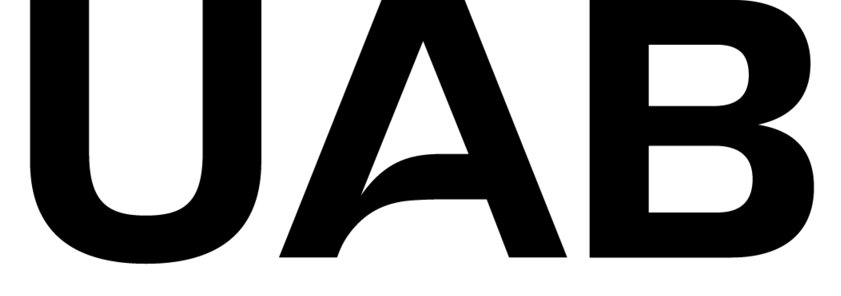
\includegraphics[width = 0.25\textwidth]{GeneralSources/UABLogo.png}\\ [0.5cm]
		\textsc{\NetIDb}\\ [2.0cm]
		\HRule{0.5pt} \\
		\LARGE \textbf{\uppercase{\documenttitle}}
		\HRule{2pt} \\ [1.5cm]
		\normalsize \begin{tabular}{rcl}  % Create a right-left column alignment
        \textsc{Author} & : & \textsc{\AuthorName} \\
        \textsc{Supervisor} & : & \textsc{Ramón Muñoz Tapia} \\
        \textsc{Co-Supervisor} & : & \textsc{Santiago Llorens Fernández}
    \end{tabular}
    \normalsize \vspace*{5\baselineskip}
		}

\date{2024-2025}

\author{\large \textsc{\subject} \\ \textsc{\degree}}



\begin{titlepage}
\clearpage\maketitle
\thispagestyle{empty}
\end{titlepage}

\thispagestyle{empty}
\mbox{} 
\newpage
\thispagestyle{empty}
\vspace*{\fill} % Push content to vertical center
\begin{flushright}
    \emph{Ab ovo usque ad mala.}\\[1em]
    \textbf{Horace}
\end{flushright}
\vspace*{\fill} 
\newpage
\thispagestyle{empty}
\mbox{} 
\newpage

\newpage
\pagestyle{fancyplain}
\headheight 35pt
\lhead{\NetIDb}    
\rhead{\subject}
\cfoot{\small\thepage}
\headsep 1.5em
\setcounter{page}{1}
\begin{multicols}{2}[\begin{center}
\begin{abstract}
Given a quantum state known to be prepared from an ensemble of two or more states, quantum state exclusion aims to rule out the possibility that it was prepared in a particular state from the ensemble. Using the known solution for group generated ensembles \cite{MainPaper}, we study this result as a lower bound for randomly generated ensembles via semidefinite programming.
\end{abstract}
\end{center}
Keywords: \emph{SDP, Quantum state exclusion , \textcolor{blue}{Add keywords}}.
]
\section{Introduction}
In many real-world scenarios, excluding a certain hypothesis can be more practical than solving the problem entirely. For instance, in disease diagnosis, ruling out potential diseases often serves as the first step in identifying the actual condition. Similarly, when repairing a machine, it is sometimes more efficient to identify the components that are functioning correctly, which narrows down the search for the faulty part.

In this project, we project this idea into the quantum realm by focusing on \gls{qse}. Rather than determining the exact state of a quantum system, we aim to eliminate one or more possible candidates from a known ensemble of states. Notice, this approach can be more suitable or efficient in certain quantum information tasks.

Given a quantum state known to be prepared from a finite ensemble, \gls{qsd} seeks to identify which specific state from the ensemble corresponds to the given system. In contrast, \gls{qse}~\cite{PhysicsExclusionSource} adopts the opposite perspective: it aims to determine which states from the ensemble do not correspond to the prepared state. While \gls{qsd} has been deeply studied in recent years\cite{DiscriminationArticle}, with significant advances since its inception~\cite{helstromBook}, \gls{qse} offers a complementary framework with distinct advantages.

Although the tasks of exclusion and discrimination coincide for ensembles containing only two states \footnote{Since for the two states case excluding one necessarily implies identifying the other.}, when dealing with ensembles of three or more states, the two problems diverge in both approach and complexity. One of the most significant features of \gls{qse} is the possibility of achieving \emph{perfect exclusion}, where certain states can be ruled out with zero probability of error in cases where \emph{perfect discrimination} is impossible\cite{OptimalitySRM}. 

This capability opens new frontiers in quantum information theory, particularly in the context of partial information retrieval from quantum systems. By excluding certain states, it is possible to gain insight into the encoded information without needing to fully determine the original state.

As with \gls{qsd}, obtaining a general analytical solution for \gls{qse} remains an open problem. However, analytical results have been found in specific cases when the ensemble of quantum states exhibits a certain degree of symmetry. In particular, when the ensemble is generated by the action of a finite group, the problem becomes more tractable and exact solutions have been derived.

The exclusion task can be carried out under two main protocols: \gls{me} and \gls{ze}\footnote{Also known as \emph{unambiguous exclusion}.}. In the Minimum Error scenario, the goal is to minimize the probability of mistakenly excluding the actual prepared state. In contrast, the Zero Error approach seeks to exclude a state with absolute certainty, even if that means sometimes the procedure yields an inconclusive result.

Building on recent results that provide exact solutions for exclusion tasks in group generated ensembles \cite{MainPaper}, this project undertakes a numerical study of such results as lower bounds for more general, randomly generated ensembles. To this end, we employ \gls{sdp} to explore \gls{qse} performance in arbitrary settings. Furthermore, we investigate improved bounds for the general case based on how closely a given ensemble resembles a group generated one\footnote{The notion of "how close" will be formally defined in Section~\textcolor{blue}{add section}.}.

\subsection{Formulation of the Problem}\label{sectionFormulationOfTheProblem}

Let $\left\{(\rho_i, \eta_i)\right\}_{i=1}^n$ be an ensemble of $n$ quantum states, where each $\rho_i$ denotes a pure state density matrix\footnote{This formulation hols true for mixed states but the project will only discuss the pure state scenario.}, i.e., $\rho_i = \ket{\psi_i}\bra{\psi_i}$, and $\eta_i$ represents the prior probability of occurrence of the state $\rho_i$. Let $\rho_j$ be the target state from this ensemble. Our objective is to develop a procedure to identify another state $\rho_k \in \left\{\rho_i\right\}_{i=1}^n$, such that $\rho_k \neq \rho_j$.

Quantum measurements are described by a set of \glspl{povm}, denoted by $\left\{\Pi_i\right\}_{i=1}^n$, acting on the Hilbert space $\mathcal{H}$ of the quantum system. Here we pewsent the two studied protocols for \gls{qse}: minimum-error (\gls{me}) and zero-error (\gls{ze}).

The goal of the \gls{me} protocol is to minimize the probability of incorrectly excluding the target state from our hypothesis. If we formulate it as an \gls{sdp}, the problem reads,\footnote{Note that the \gls{sdp} formulations of quantum state discrimination may differ from the exclusion ones by interchanging minimization and maximization problems.}
\begin{align*}
	P_{\text{\gls{me}}}^e = \min_{\left\{\Pi_i\right\}} &\sum_{i=1}^n \tr(\Pi_i \rho_i),\\
	\text{subject to} \quad & \sum_{i=1}^n \Pi_i = \mathds{1}, \quad \Pi_i \geq 0 \quad \forall i \in \{1, \dots, n\}.
\end{align*}

Note the constraints $\sum_{i=1}^n \Pi_i = \mathds{1}$ and $\Pi_i \geq 0$ ensure that the $\Pi_i$ form a valid POVM, since they demand positive semi-definition and form a complete measurement. The superscript $e$ in $P_{\text{\gls{me}}}^e$ indicates that this is the \emph{error probability}.

Alternatively, we may formulate the problem in terms of the \emph{success probability}, denoted by $P_{\text{\gls{me}}}^s$, which quantifies the probability of a correct exclusion. This equivalent formulation reads,
\begin{align*}
	P_{\text{\gls{me}}}^s = \max_{\left\{\Pi_i\right\}} &\left(1 - \sum_{i=1}^n \tr(\Pi_i \rho_i)\right),\\
	\text{subject to} \quad & \sum_{i=1}^n \Pi_i = \mathds{1}, \quad \Pi_i \geq 0 \quad \forall i \in \{1, \dots, n\}.
\end{align*}

Naturally, both formulations are related via:
\begin{align*}
P_{\text{\gls{me}}}^s + P_{\text{\gls{me}}}^e = 1.
\end{align*}

In the case of the \gls{ze} protocol, the POVMs must also satisfy an unambiguity condition, i.e. each measurement operator $\Pi_i$ must be orthogonal to the corresponding state $\rho_i$. In other words,
\begin{align*}
\tr(\Pi_i \rho_i) = 0 \quad \forall i \in \{1, \dots, n\}.
\end{align*}

To ensure completeness, we introduce an additional POVM element $\Pi_?$ representing an inconclusive result,
\begin{align*}
\Pi_? = \mathds{1} - \sum_{i=1}^n \Pi_i.
\end{align*}
If the measurement yields the outcome $\Pi_?$ (i.e., the "?" symbol), the result is inconclusive.

The corresponding \gls{sdp} for minimizing the probability of an inconclusive result (i.e., error) in the \gls{ze} protocol is:
\begin{align*}
	P_{\text{\gls{ze}}}^e = \min_{\left\{\Pi_i\right\}} &\sum_{i=1}^n \tr(\Pi_? \rho_i),\\
	\text{subject to} \quad & \sum_{i=1}^n \Pi_i + \Pi_? = \mathds{1}, \quad \Pi_? \geq 0,\\
	& \tr(\Pi_i \rho_i) = 0, \quad \Pi_i \geq 0 \quad \forall i.
\end{align*}

The corresponding success probability is naturally given by,
\begin{align*}
	P_{\text{\gls{ze}}}^s = \max_{\left\{\Pi_i\right\}} &\left(1 - \sum_{i=1}^n \tr(\Pi_? \rho_i)\right),\\
	\text{subject to} \quad & \sum_{i=1}^n \Pi_i + \Pi_? = \mathds{1}, \quad \Pi_? \geq 0,\\
	& \tr(\Pi_i \rho_i) = 0, \quad \Pi_i \geq 0 \quad \forall i.
\end{align*}

This formulation is analogous to the \gls{me} protocol, with the crucial difference being the constraint $\tr(\Pi_i \rho_i) = 0$, enforcing unambiguous discrimination.

\subsection{Gram Matrix Formulation}\label{sectionGramMatrixFormulation}

Let $\mathcal{G} \in \mathbb{C}^{n \times n}$ be the \emph{Gram matrix} of the system, defined as the $n \times n$ positive semidefinite Hermitian matrix given by,
\begin{equation*}
	\mathcal{G} =
	\begin{pmatrix}
		\braket{\psi_1|\psi_1} & \braket{\psi_1|\psi_2} & \dots & \braket{\psi_1|\psi_n} \\
		\braket{\psi_2|\psi_1} & \braket{\psi_2|\psi_2} & \dots & \braket{\psi_2|\psi_n} \\
		\vdots & \vdots & \ddots & \vdots \\
		\braket{\psi_n|\psi_1} & \braket{\psi_n|\psi_2} & \dots & \braket{\psi_n|\psi_n}
	\end{pmatrix},
\end{equation*}
that is, $\mathcal{G}_{i,j} = \braket{\psi_i|\psi_j}$. Since all states are normalized, the diagonal elements are equal to 1, and the Gram matrix becomes,
\begin{equation*}
	\mathcal{G} =
	\begin{pmatrix}
		1 & \braket{\psi_1|\psi_2} & \dots & \braket{\psi_1|\psi_n} \\
		\braket{\psi_2|\psi_1} & 1 & \dots & \braket{\psi_2|\psi_n} \\
		\vdots & \vdots & \ddots & \vdots \\
		\braket{\psi_n|\psi_1} & \braket{\psi_n|\psi_2} & \dots & 1
	\end{pmatrix}.
\end{equation*}

By construction, the Gram matrix is Hermitian,
\begin{align*}
	\mathcal{G}_{i,j}^* = (\braket{\psi_i|\psi_j})^* = \braket{\psi_j|\psi_i} = \mathcal{G}_{j,i}.
\end{align*}
Additionally, $\mathcal{G}$ is positive semidefinite. To see this, consider an arbitrary state $\ket{\Phi}$ and an orthonormal basis $\{\ket{i}\}_{i=1}^n$, then,
\begin{align*}
	\braket{\Phi|\mathcal{G}|\Phi} &= \braket{\Phi| \left( \sum_{i,j=1}^{n} \braket{\psi_i|\psi_j} \ket{i}\bra{j} \right) |\Phi} \\
	&= \sum_{i,j=1}^{n} \braket{\psi_i|\psi_j} \braket{\Phi|i} \braket{j|\Phi} \\
	&= \left\| \sum_{i=1}^{n} \braket{i|\Phi} \ket{\psi_i} \right\|^2 \\
	&\geq 0.
\end{align*}

The Gram matrix allows us to reformulate the exclusion problem in a more abstract, basis-independent manner. Since $\mathcal{G}$ is Hermitian and positive semidefinite, it can be factorized as,
\begin{align*}
	\mathcal{G} = X^\dagger X,
\end{align*}
for some matrix $X$, whose columns are the pure states,
\begin{align*}
	X = \begin{pmatrix}
		\mid & \mid &        & \mid \\
		\ket{\psi_1} & \ket{\psi_2} & \dots & \ket{\psi_n} \\
		\mid & \mid &        & \mid
	\end{pmatrix}.
\end{align*}

Let us fix an arbitrary orthonormal basis $\{\ket{\omega_i}\}_{i=1}^n$. Then, the diagonal entries of $X$ in this basis are given by,
\begin{align*}
	X_{i,i} = \braket{\omega_i|\psi_i}.
\end{align*}
\footnote{Note that fixing the basis $\{\ket{\omega_i}\}_{i=1}^n$ uniquely determines the decomposition $\mathcal{G} = X^\dagger X$, and vice versa.}We define the POVM elements as projectors $\Pi_i = \ket{\omega_i}\bra{\omega_i}$. Then, for the ensemble $\{(\rho_i, \eta_i)\}_{i=1}^n$, the corresponding semidefinite program (\gls{sdp}) constraints become,
\begin{align*}
	\tr(\Pi_i \rho_i) &= \tr\left( \ket{\omega_i}\bra{\omega_i} \ket{\psi_i}\bra{\psi_i} \right) \\
	&= |\braket{\omega_i|\psi_i}|^2 \\
	&= |X_{i,i}|^2.
\end{align*}

Thus, we can reformulate the \gls{sdp} for the minimum-error (\gls{me}) protocol as,
\begin{align*}
	P_{\gls{me}}^e = \min_{X} &\sum_{i=1}^n \frac{|X_{i,i}|^2}{\eta_i}, \\
	\text{subject to} \quad & X^\dagger X = \mathcal{G}, \quad X \geq 0.
\end{align*}

Similarly, the success probability becomes,
\begin{align*}
	P_{\gls{me}}^s = \max_{X} &\left( 1 - \sum_{i=1}^n \frac{|X_{i,i}|^2}{\eta_i} \right), \\
	\text{subject to} \quad & X^\dagger X = \mathcal{G}, \quad X \geq 0.
\end{align*}

This reformulation reveals that if two ensembles $A$ and $B$ share the same Gram matrix, then their exclusion problems under both the \gls{me} and \gls{ze} protocols are equivalent. That is, their optimal success and error probabilities coincide. Consequently, we focus on the Gram matrix to study exclusion problems rather than the explicit state representations.

Furthermore, we note that the case of arbitrary prior probabilities $\eta_i$ can be reduced to the equal prior case $\eta_i = \frac{1}{n}$ by defining non-normalized states,
\begin{align*}
	\ket{\tilde{\psi}_i} = \frac{1}{\sqrt{\eta_i}} \ket{\psi_i},
\end{align*}
and reformulating the problem in terms of these states. The prior probabilities are then absorbed into the state norm. Therefore, without loss of generality, in this project we will assume equal prior probabilities.

\subsection{Group Generated Ensembles}\label{sectionGroupGeneratedEnsemble}

Given a quantum state $\ket{\psi}$, referred to as the \emph{seed state}, we define a \emph{group generated ensemble} as the set of states obtained by applying a group of unitary transformations to $\ket{\psi}$. Specifically, if the ensemble consists of $n$ quantum states, its elements are of the form
\begin{align*}
	U_i\ket{\psi}, \quad i \in \{1, \dots, n\},
\end{align*}
where the set of unitary matrices $\{U_i\}_{i=1}^n$ forms a finite group under standard matrix multiplication. In terms of density matrices, the ensemble can equivalently be written as,
\begin{align*}
	\rho_i = U_i \rho U_i^\dagger, \quad i \in \{1, \dots, n\},
\end{align*}
where $\rho = \ket{\psi}\bra{\psi}$ is the density matrix corresponding to the seed state.

For instance, let $\mathcal{U}$ be a unitary operator such that $\mathcal{U}^n = \mathds{1}$ (i.e., $\mathcal{U}$ generates a cyclic group of order $n$). Then, the set of states
\begin{align*}
	\left\{ \mathcal{U}^i\ket{\psi} \right\}_{i=0}^{n-1},
\end{align*}
forms a group generated ensemble based on the cyclic group $\mathbb{Z}/n\mathbb{Z}$. This type of ensemble is of particular interest in our study and will be explored in more detail in a subsequent section.

\emph{Example: The $\mathbb{Z}/n\mathbb{Z}$ group-generated ensemble}: Let $\mathcal{U} \in U(n)$ be an $n \times n$ unitary matrix satisfying $\mathcal{U}^n = \mathds{1}$, and let $\ket{\psi}$ be the seed state. The Gram matrix $\mathcal{G}^{\mathbb{Z}/n\mathbb{Z}}$ elements associated with the ensemble $\left\{\mathcal{U}^i\ket{\psi}\right\}_{i=0}^{n-1}$ are
\begin{align*}
	\mathcal{G}^{\mathbb{Z}/n\mathbb{Z}}_{i,j} = \braket{\mathcal{U}^i\psi | \mathcal{U}^j\psi} = \braket{\psi | \mathcal{U}^{j-i} | \psi} = \braket{\mathcal{U}^{j-i}}_{\psi},
\end{align*}
where we use the shorthand notation,
\begin{align*}
	\braket{\mathcal{U}^k}_\psi := \braket{\psi | \mathcal{U}^k | \psi}.
\end{align*}

Using this, the Gram matrix $\mathcal{G}^{\mathbb{Z}/n\mathbb{Z}}$ can be expressed as a circulant matrix,
\begin{align*}
	\mathcal{G}^{\mathbb{Z}/n\mathbb{Z}} = \begin{pmatrix}
 1 & \braket{\mathcal{U}}_{\psi} & \braket{\mathcal{U}^2}_{\psi} & \cdots & \braket{\mathcal{U}^{n-1}}_{\psi} \\
 \braket{\mathcal{U}^{n-1}}_{\psi}^* & 1 & \braket{\mathcal{U}}_{\psi} & \cdots & \braket{\mathcal{U}^{n-2}}_{\psi} \\
 \braket{\mathcal{U}^{n-2}}_{\psi}^* & \braket{\mathcal{U}^{n-1}}_{\psi}^* & 1 & \cdots & \braket{\mathcal{U}^{n-3}}_{\psi} \\
 \vdots & \vdots & \vdots & \ddots & \vdots \\
 \braket{\mathcal{U}}_{\psi}^* & \braket{\mathcal{U}^{2}}_{\psi}^* & \braket{\mathcal{U}^{3}}_{\psi}^* & \cdots & 1
\end{pmatrix}.
\end{align*}

Note that the Gram matrix is Hermitian, as expected, since
\begin{align*}
    \braket{\mathcal{U}^{-j}}_{\psi} = \braket{\psi | \mathcal{U}^{-j} | \psi} = \left(\braket{\psi | \mathcal{U}^j | \psi}\right)^* = \braket{\mathcal{U}^j}_{\psi}^*.
\end{align*}
Additionally, by using the identity $\mathcal{U}^n = \mathds{1}$, we can simplify expressions such as,
\begin{align*}
	\braket{\mathcal{U}^{-n+i}}_\psi = \braket{\psi | \mathcal{U}^{-n+i} | \psi} = \braket{\psi | \mathcal{U}^i | \psi} = \braket{\mathcal{U}^i}_\psi.
\end{align*}
Thus, we may write,
\begin{align*}
	\mathcal{G}^{\mathbb{Z}/n\mathbb{Z}}_{\psi} = \begin{pmatrix}
 1 & \braket{\mathcal{U}}_{\psi} & \braket{\mathcal{U}^{2}}_{\psi} & \hdots &  \braket{\mathcal{U}}_{\psi}^* \\
 \braket{\mathcal{U}}_{\psi}^* & 1 & \braket{\mathcal{U}}_{\psi} & \hdots &  \braket{\mathcal{U}^{2}}_{\psi}^* \\
 \braket{\mathcal{U}^{2}}_{\psi}^* & \braket{\mathcal{U}}_{\psi}^* & 1 & \hdots &  \braket{\mathcal{U}^{3}}_{\psi}^* \\
 \vdots & \vdots & \vdots & \ddots & \vdots \\
 \braket{\mathcal{U}}_{\psi} & \braket{\mathcal{U}^{2}}_{\psi} & \braket{\mathcal{U}^{3}}_{\psi} & \hdots & 1 
\end{pmatrix}.
\end{align*}

This shows the circulant structure of $\mathcal{G}$, where each row is a cyclic permutation of the previous one. In other words, the Gram matrices of $\mathbb{Z}/n\mathbb{Z}$-generated ensembles are circulant matrices. This structure is particularly useful, as circulant matrices can be diagonalized by the discrete Fourier basis, greatly simplifying many computations~\cite{circulantMatrices}.

The Fourier basis for an $n \times n$ circulant matrix consists of the set of vectors $\{\omega_i\}_{i=1}^n$, where
\begin{align*}
	\omega_i = \frac{1}{\sqrt{n}} (1, \gamma^i, \gamma^{2i}, \ldots, \gamma^{i(n-1)})^T,
\end{align*}
and
\begin{align*}
	\gamma = e^{\frac{2\pi i}{n}}.
\end{align*}

Moreover, we can compute the Gram matrix for any group-generated ensemble by using the Cayley table~\cite{CayleyTable}, also known as the \emph{multiplication table}, of the group. For example, consider the smallest non-commutative group, $S_3$, consisting of the symmetries and rotations of an equilateral triangle. Denoting the identity as $e$, the rotations elements as $s$, $s^2$ (one being the result of 2 times the other) and the symmetries $p$, $q$, and $r$, the Cayley table is,

\begin{table}[H]
	\centering
	\caption{Cayley table of the $S_3$ group.}
	\begin{tabular}{c||c c c c c c}
        $S_3$ & $e$ & $s$ & $s^2$ & $p$ & $q$ & $r$ \\\hline\hline
        $e$   & $e$ & $s$ & $s^2$ & $p$ & $q$ & $r$ \\
        $s^2$ & $s^2$ & $e$ & $s$ & $r$ & $p$ & $q$ \\
        $s$   & $s$ & $s^2$ & $e$ & $q$ & $r$ & $p$ \\
        $p$   & $p$ & $r$ & $q$ & $e$ & $s^2$ & $s$ \\
        $q$   & $q$ & $p$ & $r$ & $s$ & $e$ & $s^2$ \\
        $r$   & $r$ & $q$ & $p$ & $s^2$ & $s$ & $e$
    \end{tabular}
\end{table}

We now identify $S_3$ as a group of unitary matrices\footnote{We treat each group element as a unitary matrix, and the group operation as matrix multiplication.}. It follows that the Gram matrix of the $S_3$ group-generated ensemble is the matrix of expected values of the Cayley table entries with respect to the seed state $\ket{\psi}$. That is,
\begin{align*}
	\mathcal{G}^{S_3}_{\psi} = \begin{pmatrix}
        1 & \braket{s}_\psi & \braket{s^2}_\psi & \braket{p}_\psi & \braket{q}_\psi & \braket{r}_\psi \\ 
        \braket{s^2}_\psi & 1 & \braket{s}_\psi & \braket{r}_\psi & \braket{p}_\psi & \braket{q}_\psi \\
        \braket{s}_\psi & \braket{s^2}_\psi & 1 & \braket{q}_\psi & \braket{r}_\psi & \braket{p}_\psi \\
        \braket{p}_\psi & \braket{r}_\psi & \braket{q}_\psi & 1 & \braket{s^2}_\psi & \braket{s}_\psi \\
        \braket{q}_\psi & \braket{p}_\psi & \braket{r}_\psi & \braket{s}_\psi & 1 & \braket{s^2}_\psi \\
        \braket{r}_\psi & \braket{q}_\psi & \braket{p}_\psi & \braket{s^2}_\psi & \braket{s}_\psi & 1
	\end{pmatrix}.
\end{align*}
Note that $\braket{e}_\psi = 1$ since $e = \mathds{1}$. Moreover, since $\mathcal{G}^{S_3}$ is Hermitian, we conclude:
\begin{align*}
\braket{p}_{\psi},\ \braket{q}_{\psi},\ \braket{r}_{\psi} \in \mathbb{R}, \quad \forall \ket{\psi} \in \mathcal{H},
\end{align*}
which implies the unitary matrices corresponding to the triangle symmetries $p$, $q$, and $r$ are Hermitian. As a matter of fact we know the eigenvalues of this matrices can only be $\pm 1$ and at least one of them must be $-1$.\footnote{Otherwise, they would be the identity and we know them to be different by construction.} This procedure generalizes to any finite group $G$, showing that computing the Cayley table is equivalent to computing the Gram matrix of the corresponding group-generated ensemble.

Finally, we denote the cardinality of a finite group $G$ (i.e., the number of its elements) as $|G|$. In scenarios with uniform prior probabilities, this implies,
\begin{align*}
	\eta_i = \frac{1}{|G|}\quad \forall i\in\{1,...,n\}.
\end{align*}
\subsection{Dual Formulation of the Problem}

It is often useful to consider the \emph{dual} version of a \gls{sdp} problem, as it provides both conceptual insights and practical advantages for verifying optimality. 

Consider the ensemble $\left\{ \left( \rho_i, \frac{1}{n} \right) \right\}_{i=1}^n$, where each state $\rho_i$ appears with uniform prior probability $1/n$. The dual SDP corresponding to the Minimum Error (\gls{me}) exclusion protocol, when expressed in terms of the error probability, is given by,
\begin{align*}
	\tilde{P}_{\gls{me}}^e = \max_{\Gamma} \quad & \tr{\Gamma} \\
	\text{subject to} \quad & \frac{\rho_i}{n} - \Gamma \geq 0 \quad \forall i \in \{1, \dots, n\}, \\
	& \Gamma^\dagger = \Gamma,
\end{align*}
where $\tilde{P}$ denotes the dual version of the problem.

Similarly, the dual SDP for the success probability in the same protocol reads:
\begin{align*}
	\tilde{P}_{\gls{me}}^s = \min_{\Gamma} \quad & 1 - \tr{\Gamma} \\
	\text{subject to} \quad & \frac{\rho_i}{n} - \Gamma \geq 0 \quad \forall i \in \{1, \dots, n\}, \\
	& \Gamma^\dagger = \Gamma.
\end{align*}

\textcolor{blue}{Add the dual version for the zero error protocol.}

In the case of the zero-error exclusion protocol, the dual SDP formulation becomes 

One of the primary uses of the dual formulation is in establishing optimality. If a POVM ansatz yields equal objective values for both the primal and dual problems, i.e., $P = \tilde{P}$, then strong duality holds and the measurement is guaranteed to be optimal.

This duality principle not only provides a tool for verification but also suggests constructive approaches to discovering optimal measurements, especially in structured ensembles such as those generated by group actions.
\subsection{Previous Results}\label{sectionPreviousResults}

Significant progress has been made in the study of the state exclusion task for group-generated ensembles. In particular, the work \emph{Quantum State Exclusion for Group-Generated Ensembles of Pure States}\cite{MainPaper} presents exact analytical expressions for the success and error probabilities under both the Minimum Error \gls{me} and Zero Error \gls{ze} exclusion protocols.

Let $\mathcal{G}^G$ denote the Gram matrix of a group-generated ensemble $\left\{ \left( \rho_i, \frac{1}{|G|} \right) \right\}_{i=1}^{|G|}$, where $G$ is a finite group of size $|G|$, and let $\{\lambda_i\}_{i=1}^{|G|}$ be the set of eigenvalues of $\mathcal{G}^G$. Assume the eigenvalues are ordered increasingly,
\begin{align*}
	i \leq j \quad \Leftrightarrow \quad \lambda_i \leq \lambda_j, \quad \forall i,j \in \{1, \dots, |G|\},
\end{align*}
i.e., $\lambda_1$ is the smallest and $\lambda_{|G|}$ the largest eigenvalue.

The exclusion probabilities under the Minimum Error protocol are given by,
\begin{align*}
	P_{\gls{me}}^e &= \max\left\{ 0, \left( \frac{ \sqrt{\lambda_{|G|}} - \sum_{i<|G|} \sqrt{\lambda_i} }{|G|} \right)^2 \right\}, \\
	P_{\gls{me}}^s &= \min\left\{ 1, 1 - \left( \frac{ \sqrt{\lambda_{|G|}} - \sum_{i<|G|} \sqrt{\lambda_i} }{|G|} \right)^2 \right\}.
\end{align*}

For the Zero Error protocol, the corresponding expressions arem
\begin{align*}
	P_{\gls{ze}}^e &= \max\left\{ 0, \frac{ \sum_{i=1}^{|G|} \sqrt{\lambda_i} \left( \sqrt{\lambda_{|G|}} - \sum_{j<|G|} \sqrt{\lambda_j} \right) }{|G|} \right\}, \\
	P_{\gls{ze}}^s &= \min\left\{ 1, 1 - \frac{ \sum_{i=1}^{|G|} \sqrt{\lambda_i} \left( \sqrt{\lambda_{|G|}} - \sum_{j<|G|} \sqrt{\lambda_j} \right) }{|G|} \right\}.
\end{align*}

A key feature of these results is their independence from the specific group generating the ensemble. That is, for any two group-generated ensembles $A$ and $B$ corresponding to groups $G_A$ and $G_B$ (with $G_A \neq G_B$ but $|G_A| = |G_B|$), if their respective Gram matrices $\mathcal{G}^{G_A}$ and $\mathcal{G}^{G_B}$ share the same eigenvalues, then the exclusion probabilities for both \gls{me} and \gls{ze} protocols are identical. This group-independence property is a cornerstone of the present study.

Another important outcome from \cite{MainPaper} is the identification of conditions under which perfect exclusion is achievable, i.e., the exclusion can be carried out with zero error. This occurs if the eigenvalues satisfy the inequality,

\begin{align}\label{equationPerfectExclusionCondition}
	\lambda_{|G|} \leq \left( \sum_{i=1}^{|G|} \sqrt{\lambda_i} \right)^2.
\end{align}

We refer to the regime satisfying this inequality as the \emph{perfect exclusion zone}. Within this regime, the success probability of the exclusion task reaches one, implying that exclusion can be performed perfectly.

In this project, we will extend this result by demonstrating that the perfect exclusion condition Eq. (\ref{equationPerfectExclusionCondition}) provides a lower bound for the success probability of exclusion even for non-group-generated ensembles. Since this bound equals 1, it implies that any ensemble whether or not group-generated that satisfies condition Eq. (\ref{equationPerfectExclusionCondition}) can achieve perfect exclusion. Thus, the perfect exclusion zone is not exclusive to group-generated ensembles, but also includes all ensembles that fulfill the given condition.

\subsection{Limit Case Scenarios}\label{sectionLimitCaseScenarios}

Let us study the Gram matrix of a limit ensemble composed of $n$ identical quantum states (i.e., the same state is repeated $n$ times in the ensemble).\footnote{This case may appear paradoxical, since there is no way to distinguish between identical states. Nevertheless, we present it as a limiting scenario.} The Gram matrix reads:
\begin{align*}
	\mathcal{G}^{\text{limit}} = \begin{pmatrix}
 1 & 1 & \cdots & 1 \\
 1 & 1 & \cdots & 1 \\
 \vdots & \vdots & \ddots & \vdots \\
 1 & 1 & \cdots & 1 \\
\end{pmatrix}.
\end{align*}

The eigenvalues of this matrix are:
\begin{align*}
	\lambda_n &= n, \\
	\lambda_{n-1} &= 0, \\
	\vdots \\
	\lambda_1 &= 0.
\end{align*}

Clearly, this set of eigenvalues does not satisfy Eq. (\ref{equationPerfectExclusionCondition}), i.e., we are in the non-perfect exclusion regime. In fact, we can interpret this ensemble as a group-generated ensemble from the \emph{trivial group},\footnote{The trivial group is the group consisting solely of the neutral/identity element.} which generates no variation.

Thus, the success and error probabilities for both the \gls{me} protocol is,
\begin{align*}
	P_{\gls{me}}^e =& \frac{1}{n},\\
	P_{\gls{me}}^s =& \frac{n-1}{n}.
\end{align*}

The intuition behind this result is clear. If there is no physical way to distinguish between states, the exclusion must be made randomly, with uniform probability. This observation also extends naturally to \gls{qsd}.

Since this is a limiting case scenario, the success probability for either \gls{qse} or \gls{qsd} must be strictly greater than $\frac{n-1}{n}$ (i.e., the error probability must be less than $\frac{1}{n}$). Notice this result holds only for the \gls{me} protocol. Otherwise, since the exclusion cannot be accomplished without ambiguity, the successfull exclusion probability for the \gls{ze} protocol is 0 for either \gls{qse} or \gls{qsd} (i.e., the error exclusion probability is 1), 
\begin{align*}
	P_{\gls{ze}}^e =& 1,\\
	P_{\gls{ze}}^s =& 0.
\end{align*}

The opposite limiting case is an ensemble of $n$ orthogonal quantum states $\{\rho_i\}_{i=1}^{n}$. In this case, the Gram matrix becomes the identity,
\begin{align*}
	\mathcal{G} = \mathds{1}.
\end{align*}

Under these conditions, both \gls{qse} and \gls{qsd} are trivial, as the states form an orthonormal basis. In particular, in the space spanned by these states, we have,
\begin{align*}
	\sum_{i=1}^{n} \rho_i = \mathds{1},
\end{align*}
which means that the set $\{\rho_i\}$ is itself a \gls{povm}. The measurement corresponding to this \gls{povm} allows perfect identification (or exclusion), hence both \gls{qse} and \gls{qsd} can be performed without error.

\subsection{Ensembles with a Prime Number of Elements}\label{sectionEnsemblesWithPrime}

As previously discussed, analytical solutions have been found for the exclusion task under both the \gls{me} and \gls{ze} protocols. These solutions depend solely on the eigenvalues of the Gram matrix and are independent of the specific group structure generating the ensemble.

Let the Gram matrix of an ensemble decompose as,
\begin{align*}
	\mathcal{G} = U D U^\dagger,
\end{align*}
where $U$ is a unitary matrix and $D$ is the diagonal matrix of eigenvalues. We then encounter two possibilities,
\begin{itemize}
	\item The eigenvalues satisfy Eq.~\eqref{equationPerfectExclusionCondition}, placing the ensemble in the \emph{perfect exclusion} regime.
	\item The eigenvalues do not satisfy Eq.~\eqref{equationPerfectExclusionCondition}, placing the ensemble in the \emph{non-perfect exclusion} regime.
\end{itemize}

In the perfect exclusion regime, the existence of a \gls{povm}, such that the measurement outcome allows exclusion of a hypothesis without error, is guaranteed.

In the non-perfect exclusion regime, the analytical results for group-generated ensembles provide lower bounds on the success probabilities (and upper bounds on the error probabilities) for general ensembles.

Consider, for example, the case of an ensemble of 4 quantum states. There are exactly two groups of four elements: $\mathbb{Z}/4\mathbb{Z}$ and $\mathbb{Z}/2\mathbb{Z} \times \mathbb{Z}/2\mathbb{Z}$.\footnote{These are the only non-isomorphic groups of order 4.} This implies that there exist two specific unitary matrices, $U_{\mathbb{Z}/4\mathbb{Z}}$ and $U_{\mathbb{Z}/2\mathbb{Z} \times \mathbb{Z}/2\mathbb{Z}}$ (up to permutation of rows and columns), for which the analytical solution holds exactly.

Since $U(n)$ is compact, and assuming continuity of the exclusion probabilities with respect to $U$ under a given matrix norm, for each of these unitary matrices there exist arbitrarily small neighborhoods $\mathcal{B}(U_{\mathbb{Z}/4\mathbb{Z}})$ and $\mathcal{B}(U_{\mathbb{Z}/2\mathbb{Z} \times \mathbb{Z}/2\mathbb{Z}})$ such that the exclusion probabilities within these neighborhoods approximate the analytical result as closely as desired. However, the existence of multiple such matrices (and intersecting neighborhoods) can complicate numerical optimization and analysis.

In contrast, it is usefull to consider the case where the ensemble contains a prime number $p$ of states. In this scenario, the situation simplifies considerably, since there exists only one group (up to isomorphism) of order $p$, namely $\mathbb{Z}/p\mathbb{Z}$.

This result follows immediately from Lagrange's theorem. The theorem guarantees that the order of any element in a finite group\footnote{The order of an element $\tau$ in a group $G$ is the smallest positive integer $m$ such that $\tau^m = e$, where $e$ denotes the identity/neutral element of the group.} must divide the order of the group. Since $p$ is a prime number, the only positive integers dividing $p$ are either $1$ or $p$ itself. Therefore, the order of any group element must be either $1$ or $p$. An element of order $1$ must be the identity, so every non-identity element in the group must have order $p$. This implies that all non-identity elements generate the entire group, i.e., the group is cyclic. As a result, any group of prime order $p$ is necessarily cyclic and isomorphic to $\mathbb{Z}/p\mathbb{Z}$.

Consequently, for an ensemble of $p$ quantum states, there exists a unique unitary matrix $U_{\mathbb{Z}/p\mathbb{Z}}$ (up to reordering) that diagonalizes the Gram matrix in such a way that the analytical results are exact. \footnote{Moreover, the columns of this matrix correspond to the elements of the Fourier basis, as discussed in Section~\ref{sectionGroupGeneratedEnsemble}, particularly in the example involving $\mathbb{Z}/n\mathbb{Z}$.}

Ensembles of prime cardinality are thus of particular interest and will be further explored in the Results and Discussion section. \textcolor{blue}{Add reference to Results section}
\section{Methodology}

All the code used in this project is hosted in the GitHub repository \cite{GitHub}, where additional documentation is available detailing the functionality and structure of each script and class involved in the implementation.

\subsection{\gls{sdp} Solver}

The core of the numerical analysis is the implementation of a Semi-Definite Programming (\gls{sdp}) solver based on the MOSEK optimization suite \cite{mosek_sdp}, interfaced through the Python-based PICOS optimization library \cite{PICOS}. 

\subsection{Generation of Random Gram Matrices}

To analyze both group-generated and generic quantum state ensembles, we developed a method for generating random Gram matrices with prescribed spectral properties.

A Numpy \gls{rng}\cite{numpyRNG} produces a set of $n$ non-negative real numbers $\{\lambda_i\}_{i=1}^n$ that are normalized to satisfy the trace condition,
\begin{align*}
	\sum_{i=1}^n \lambda_i = n.
\end{align*}
These values are used as the eigenvalues of the Gram matrix, forming the diagonal matrix $D = \operatorname{diag}(\lambda_1, \dots, \lambda_n)$. 

Next, we generate a unitary matrix $U$ and construct the Gram matrix as,
\begin{align*}
	\mathcal{G} = U D U^\dagger.
\end{align*}

At this point, we choose whether the ensemble is to be group-generated or generic.

For a generic ensemble, the unitary matrix $U$ is drawn randomly according to the Haar measure \cite{haarMeasure}, which defines the unique uniform probability measure on the unitary group $U(n)$ that is invariant under group multiplication. To ensure this uniformity, we use the algorithm introduced by Francesco Mezzadri in \cite{UnitaryMatricesGeneration}, which provides an efficient and accurate way of sampling unitary matrices while uniformly covering $U(n)$.

In the case of a group-generated ensemble, we restrict ourselves to ensembles generated by the cyclic group $\mathbb{Z}/n\mathbb{Z}$. The corresponding unitary matrix $U$ is constructed such that its columns are the vectors of the discrete Fourier basis, as discussed in Section~\ref{sectionGroupGeneratedEnsemble} (\emph{Group-Generated Ensemble}).

Other groups are omitted in our analysis since we can always choose $n$ to be a prime number, in which case the only group of order $n$ (up to isomorphism) is the cyclic group $\mathbb{Z}/n\mathbb{Z}$. This significantly simplifies the group structure and ensures that the only group-generated ensemble under consideration corresponds to a well-defined, unique construction.

This methodology provides a flexible yet rigorous foundation for both exploring generic quantum ensembles and benchmarking them against analytically tractable group-generated cases.

\section{Results and Discussion}

Let us analyze the case of a $\mathbb{Z}/3\mathbb{Z}$ ensemble. The Gram matrix in this case takes the form,
\begin{align*}
	\mathcal{G}^{\mathbb{Z}/3\mathbb{Z}}=\begin{pmatrix}
		1 & c & c^*\\
		c^* & 1 & c\\
		c & c^* & 1
	\end{pmatrix}
\end{align*}
with $c \in \mathbb{C}$. Note that, with respect to previous notation, we write $c = \braket{U}_{\psi}$, where $c$ and $c^*$ denote the overlap between different states. We can parametrize $c$ as $c = |c|e^{i\phi}$, and since we are analyzing normalized states,
\begin{align*}
	|c|\in [0,1], \quad \phi\in[0,2\pi]
\end{align*}
we observe two \gls{dof}.

Since 3 is a prime number, the only group of order 3 is $\mathbb{Z}/3\mathbb{Z}$, as discussed in Section (\ref{sectionEnsemblesWithPrime}). The Gram matrix can be diagonalized as,
\begin{align*}
	\mathcal{G}^{\mathbb{Z}/3\mathbb{Z}} = U_{\mathbb{Z}/3\mathbb{Z}} D U_{\mathbb{Z}/3\mathbb{Z}}^\dagger,
\end{align*}
where $U_{\mathbb{Z}/3\mathbb{Z}}$ is the unitary matrix with Fourier basis vectors as columns. The eigenvalues of the matrix are denoted as $\{\lambda_1,\lambda_2,\lambda_3\}$ with $\lambda_1 \leq \lambda_2 \leq \lambda_3$. Since,
\begin{align*}
	\tr(\mathcal{G}^{\mathbb{Z}/3\mathbb{Z}}) = \tr(D) = \sum_{i=1}^3 \lambda_i = 3
\end{align*}
we again find only two \glspl{dof}, consistent with our earlier parameterization. Furthermore, since $\mathcal{G}^{\mathbb{Z}/3\mathbb{Z}} \geq 0$, we have,
\begin{align*}
	\lambda_i \geq 0 \quad \forall i \in \{1,2,3\},
\end{align*}
implying the eigenvalues must lie in the interval $[0,3]$.\footnote{In general, eigenvalues lie in $[0,n]$ for an $n$-dimensional ensemble, even for non-group-generated ensembles.} Therefore,
\begin{align*}
	\lambda_3 \in [0,3], \quad \lambda_2 \in [0,\lambda_3], \quad \lambda_1 = 3 - \lambda_2 - \lambda_3.
\end{align*}

This scenario is particularly interesting as it is the only ensemble with a small enough dimension to fully visualize all parameter dependencies and study the ensemble structure.\footnote{Visualizations include two parameters along with the success/exclusion probability of the respective protocol.} Higher-dimensional cases are too complex for full representation, while two-state cases reduce to standard quantum state discrimination (\gls{qsd}) as previously discussed.

\subsection{Comparison \gls{qsd} vs. \gls{qse}, and \gls{me} vs. \gls{ze}}

We first present results for the Quantum State Discrimination (\gls{qsd}) task to motivate the problem and highlight contrasts with the Quantum State Exclusion (\gls{qse}) task, which is the focus of this study.

Figure (\ref{FigureQSDMEZ3ZHeatmap}) shows a heatmap of the average successful discrimination probability under the Minimum Error (\gls{me}) protocol for a $\mathbb{Z}/3\mathbb{Z}$ group-generated ensemble. Probabilities are shown as functions of the modulus ($x$-axis) and phase ($y$-axis) of the overlap $c$, which fully determine the Gram matrix. We assume equal prior probabilities, as generalization to arbitrary priors is discussed in Section (\ref{sectionGramMatrixFormulation}). Note, equal priors are presuposed throughout this work unless stated otherwise.

The colorless regions correspond to parameters where $\mathcal{G}^{\mathbb{Z}/3\mathbb{Z}}$ is not positive semi-definite, and leading up yo non-valid Gram matrices, since positive semi-definition is inherent to a Gram matrix.

\begin{figure}[H]
	\centering
	\label{FigureQSDMEZ3ZHeatmap}
	\begin{overpic}[width=0.5\textwidth, trim={2.3cm 0.8cm 4.5cm 2cm}, clip]{../Plots/DiscriminationOverlapVSPhaseVSMinimumErrorProbabilityZ3HeatMap.pdf}
		\put(60,25){$\mathcal{G}^{\mathbb{Z}/3\mathbb{Z}}<0$}
		\put(60,55){$\mathcal{G}^{\mathbb{Z}/3\mathbb{Z}}<0$}
	\end{overpic}
	\caption{Heatmap of the success probability for minimum error (\gls{me}) quantum state discrimination for a $\mathbb{Z}/3\mathbb{Z}$ group-generated ensemble.}
\end{figure}

In these conditions, the \gls{srm}\footnote{Also known as the Pretty Good Measurement.} is optimal, i.e. the result of the \gls{sdp} matches the one obtained from the \gls{srm}. In particular, the \gls{srm} is obtained from the square root decomposition of the Gram matrix,
\begin{align*}
	\mathcal{G} = S^\dagger S = S^2
\end{align*}
and is the standard in \gls{qsd} under the \gls{me} protocol \cite{OptimalitySRM}.

As expected, no ensemble yields a success probability below $1/3$, consistent with the discussion in Section (\ref{sectionLimitCaseScenarios}). Moreover, as the modulus of the overlap approaches zero, the success probability approaches one, corresponding to orthogonal states, again matching expectations.

Figure (\ref{FigureQSDZEZ3ZHeatmap}) shows results for the Zero Error (\gls{ze}) protocol under the same conditions.

\begin{figure}[H]
	\centering
	\label{FigureQSDZEZ3ZHeatmap}
	\begin{overpic}[width=0.5\textwidth, trim={2.3cm 0.8cm 4.5cm 2cm}, clip]{../Plots/DiscriminationOverlapVSPhaseVSSuccessProbabilityZeroErrorZ3HeatMap.pdf}
		\put(60,25){$\mathcal{G}^{\mathbb{Z}/3\mathbb{Z}}<0$}
		\put(60,55){$\mathcal{G}^{\mathbb{Z}/3\mathbb{Z}}<0$}
	\end{overpic}
	\caption{Heatmap of the success probability for zero-error (\gls{ze}) quantum state discrimination for a $\mathbb{Z}/3\mathbb{Z}$ group-generated ensemble.}
\end{figure}

Both limiting behaviors remain valid. However, the \gls{ze} success probabilities are lower than those of the \gls{me} protocol. This is explained by the stricter constraints imposed in the \gls{ze} scenario, where $\tr(\Pi_i\rho_i) = 0$ is enforced for all POVM elements except one. Notice both probabilities are computed in a completely symmetric way,
\begin{align*}
	P^s_{\gls{me}}\sim P^s_{\gls{ze}}\sim 1-\sum_{\gls{povm}}\tr{(\Pi_i\rho_i)}.
\end{align*}

Nevertheless, in the \gls{ze} case we enforce $\tr{(\Pi_i\rho_i)}=0$ for all the \glspl{povm} except one. Thus, the system is more constrained in the \gls{ze} protocol, then the optimization of the probability cannot be performed up to the same point as in the \gls{me} protocol. Hence, the success probabilities for \gls{me} are greater than the ones obtained with the \gls{ze} protocol.

Figure (\ref{FigureQSDMEZESRM}) compares the performance of the ME, ZE, and SRM protocols.

\begin{figure}[H]
	\centering
	\label{FigureQSDMEZESRM}
	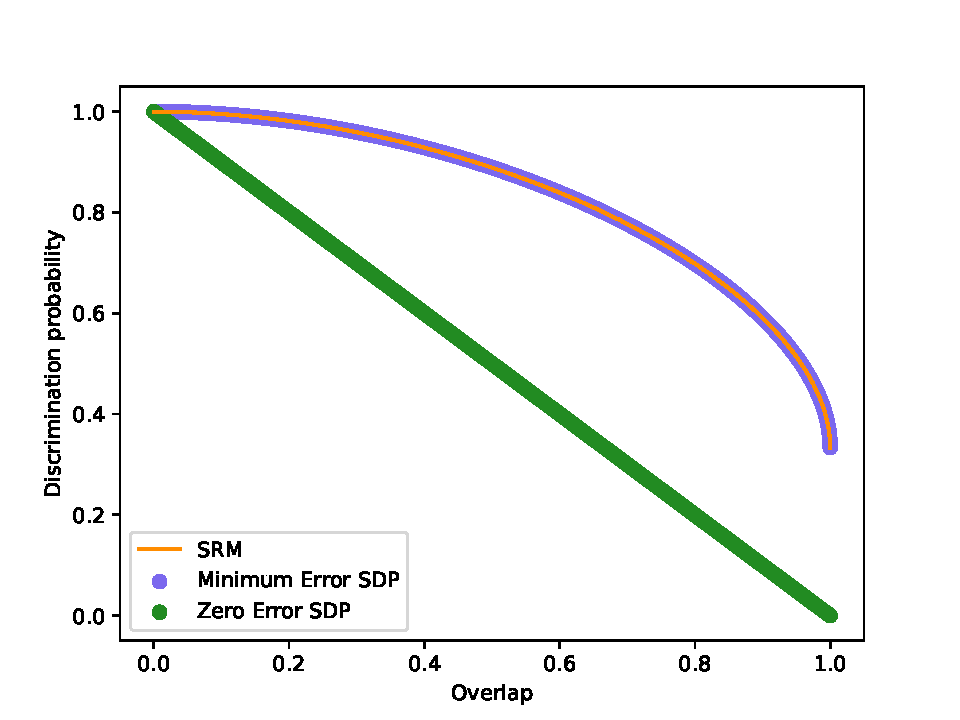
\includegraphics[width=0.5\textwidth]{../Plots/DiscriminationOverlapVSSucessProbabilitySDPvsSRMZnOverlap3Phase0.pdf}
	\caption{Comparison of successful discrimination probabilities for ME, ZE, and SRM protocols in a $\mathbb{Z}/3\mathbb{Z}$ ensemble impossing phase=$0$.}
\end{figure}

As expected, perfect discrimination is only achieved when the overlap is zero (orthogonal states), and the \gls{srm} success probability matches the one obtained from the numerical \gls{sdp}. This highlights the motivation behind the study of \gls{qse}, which allows for perfect exclusion in cases where discrimination is impossible.

\begin{figure}[H]
	\centering
	\label{FigureQSEMEZ3ZHeatmap}
	\begin{overpic}[width=0.5\textwidth, trim={2.3cm 0.8cm 4.5cm 2cm}, clip]{../Plots/ExlusionOverlapVSPhaseVSMinimumErrorProbabilityZ3HeatMap.pdf}
		\put(60,25){$\mathcal{G}^{\mathbb{Z}/3\mathbb{Z}}<0$}
		\put(60,55){$\mathcal{G}^{\mathbb{Z}/3\mathbb{Z}}<0$}
	\end{overpic}
	\caption{Heatmap of the success probability for minimum error (\gls{me}) quantum state exclusion in a $\mathbb{Z}/3\mathbb{Z}$ ensemble.}
\end{figure}

Figure (\ref{FigureQSEMEZ3ZHeatmap}) presents the ME protocol results for the \gls{qse} task, analogous to Figure (\ref{FigureQSDMEZ3ZHeatmap}).

The ZE protocol for \gls{qse} is shown in Figure (\ref{FigureQSEZEZ3ZHeatmap}).

\begin{figure}[H]
	\centering
	\label{FigureQSEZEZ3ZHeatmap}
	\begin{overpic}[width=0.5\textwidth, trim={2.3cm 0.8cm 4.5cm 2cm}, clip]{../Plots/ExlusionOverlapVSPhaseVSZeroErrorProbabilityZ3HeatMap.pdf}
		\put(60,25){$\mathcal{G}^{\mathbb{Z}/3\mathbb{Z}}<0$}
		\put(60,55){$\mathcal{G}^{\mathbb{Z}/3\mathbb{Z}}<0$}
	\end{overpic}
	\caption{Heatmap of the success probability for zero-error (\gls{ze}) quantum state exclusion in a $\mathbb{Z}/3\mathbb{Z}$ ensemble.}
\end{figure}

\begin{figure}[H]
	\centering
	\label{FigureQSEMEZ3ZPerfectExclusion}
	\begin{overpic}[width=0.5\textwidth, trim={2.3cm 0.8cm 2.5cm 2cm}, clip]{../Plots/ExlusionOverlapVSPhaseVSPerfectExclussionZoneZ3BinaryHeatMap.pdf}
		\put(70,27){$\mathcal{G}^{\mathbb{Z}/3\mathbb{Z}}<0$}
		\put(70,60){$\mathcal{G}^{\mathbb{Z}/3\mathbb{Z}}<0$}
	\end{overpic}
	\caption{Perfect exclusion zone for a $\mathbb{Z}/3\mathbb{Z}$ ensemble under the minimum error (\gls{me}) protocol.}
\end{figure}

Again, the ZE protocol yields lower probabilities due to its constraints and the limit case scenarios match with the previos discussion in Section (\ref{sectionLimitCaseScenarios}). However, crucially, perfect exclusion is possible even when perfect discrimination is not, in this regime seems to correspond to the ensembles such that the modulus of the overlap between two ensembles do not overtakes $\frac{1}{2}$. Nevertheless, this description is purely observational, we will give a better description in Section (\ref{sectionPerfectExclusionRegimeAndGeneralEnsembles}). Notice Figure (\ref{FigureQSEMEZ3ZPerfectExclusion}) highlights the regions where perfect exclusion is achieved, even outside the perfect discrimination regime.

This property of \gls{qse} is a major motivation for its study. For example, in a regime where perfect exclusion is possible, having access to multiple copies of a target state enables hybrid exclusion-discrimination protocols that can outperform purely discriminative strategies. Even partial information, such as the exclusion of a single quantum state, has value in certain quantum information theories. These features make \gls{qse} a fertile ground for further theoretical and applied research.

\subsection{The perfect exclusion regime and general ensembles}\label{sectionPerfectExclusionRegimeAndGeneralEnsembles}

Although the $Overlap modulus - phase$ spectrum might seem as the most intuituve representation, the spectrum of Gram's matrix eigenvalues results the most appropriate representation for the perfect exclusion zone as well as the discussion and its comparison for general ensembles. Carrying on with the previos discussion, one can check the two \gls{dof} now appear as two of the eigenvalues. In the Figure (\ref{FigureQSEMEZ3ZEigenValues}) the results for the exclusion task under the \gls{me} protocol for the $\mathbb{Z}/3\mathbb{Z}$ group-generated ensemble are represented. The axis represent two of the eigenvalues of the Gram matrix and a heatmap presents the probability for a perfect exclusion in the given conditions.

\begin{figure}[H]
	\centering
	\label{FigureQSEMEZ3ZEigenValues}
	\begin{overpic}[width=0.5\textwidth, trim={2.3cm 0.8cm 4.4cm 2cm}, clip]{../Plots/ExclusionEignevaluesGroupGeneratedLowerBoundZ3.pdf}
		\put(20,25){\footnotesize{Perfect exclusion}}
		\put(50,50){$\mathcal{G}^{\mathbb{Z}/3\mathbb{Z}}<0$}
	\end{overpic}
	\caption{Plot of the success exclusion probability in the eigenvalues spectrum for the \gls{me} protocol for a $\mathbb{Z}/3\mathbb{Z}$ group-generated ensemble.}
\end{figure}

The order in eigenvalues is obviated in the representation, i.e. we can find conditions such that $\lambda_i>\lambda_j$ and others conditions such that $\lambda_i<\lambda_j$ for $i,j\in\{1,2,3\}$

Notice the missing eigenvalue is determined by the other two via,
\begin{align*}
	\lambda_3=3-\lambda_1-\lambda_2.
\end{align*}
Since the Gram matrix is a positive semidefinite matrix we know that $\lambda_3\geq0$, the limit case scenario $\lambda_3=0$ defines the line,
\begin{align*}
\lambda_2=3-\lambda_1,
\end{align*}
that constraints the possible eigenvalues to only reach values under this line. Otherwise the remaining value would be negative leading up to non-valid Gram matrices as discussed in the previos plots. Naturally, we also know $\lambda_1,\lambda_2>0$, then the region $\Omega$ where the system leads up to consistent Gram matrices is,
\begin{align*}
	\Omega=\left\{(\lambda_1,\lambda_2)\in\mathbb{R}^2\left|\lambda_1\geq0,\lambda_2\geq0,\lambda_1+\lambda_2\leq3\right.\right\}.
\end{align*}
This region $\Omega$ is depicted in the Figure (\ref{FigureQSEMEZ3ZEigenValues}) as boottom left triangle, where our system is recluded. Inside this region we can find the perfect exclusion zone, i.e. the eigenvalues such that Eq.(\ref{equationPerfectExclusionCondition}) is fulfilled. In particular,if we set $\lambda_i$ with $i\in\{1,2,3\}$ to be the greatest eigenvalues and denote $\lambda_j,\lambda_k$ as the remaining 2 eigenvalues, we know perfect exclusion to be archived if,
\begin{align*}
	\sqrt{\lambda_i}\leq \sqrt{\lambda_j}+\sqrt{\lambda_k}.
\end{align*}
With a little bit of algebra and recalling that $\lambda_3=3-\lambda_1-\lambda_2$ we can derive the regime of perfect exclusion denoted as $\Delta$ comprehends the eigenvalues such that,
\begin{align*}
	(\lambda_1,\lambda_2&)\in \Delta\\
	\Updownarrow& \\
	4\lambda_1^2 + 4\lambda_2^2 + 4\lambda_1\lambda_2 - &12\lambda_1 - 12\lambda_i + 9 \leq 0
\end{align*}
Figure (\ref{FigurePerfectExclusionZ3Z}) shows the $\Delta$ region. It is inmediate that this region corresponds to the colorless perfect exclusion regime in Figure (\ref{FigureQSEMEZ3ZEigenValues}).
\begin{figure}[H]
	\centering
	\label{FigurePerfectExclusionZ3Z}
	\begin{overpic}[width=0.5\textwidth, trim={1.8cm 0.8cm 2cm 2cm}, clip]{GeneralSources/PerfectExclusionZoneZ3Z.pdf}
	\end{overpic}
	\caption{Plot of the $\Delta$ region.}
\end{figure}

Naturally we can prove the perfect exclusion zone to be a subset of valid Gram matrixes i.e. $\Delta\subset \Omega$.Then the non-perfect exclusion regime is the remaining part of the triangle i.e.,
\begin{align*}
	\text{Non-perfect exclusion regime}=\Omega\setminus \Delta.
\end{align*}
The limit case scenarios corresponding to $\lambda_i=3$ and $\lambda_j,\lambda_k=0$ are situated in the vertex of the triangle\footnote{Remember this case correspond to sets with the same state repeated 3 times discussed in Section (\ref{sectionLimitCaseScenarios})}. Then the cases corresponding to the edges are those with one state repeated 2 times and one different from the other 2. This ensembles can also be underestood as a limit case scenario systems.

In practice this scenario is entirely equivalent to a 2 quantum states exclusion (\gls{qse}) system. Nevertheless we know this to be equivalent to a 2 quantum states discrimination system (\gls{qsd}), therefore perfect discrimination/exclusion cannot be archived unless the states are orthogonal. This last case corresponds to the intersection of the elipse $\Delta$ with the triangles edges, this can be described as the ensembles with associated Gram matrices whose eigenvalues $\lambda_i,\lambda_j,\lambda_k$ are,
\begin{align*}
	\lambda_i=&\lambda_j=\frac{3}{2}\\
	\lambda_k=&0.
\end{align*}

Additionally, we observe that no ensembles seem to have a lower exclusion success probability $P_{\gls{me}}^s$ under $\frac{1}{3}$ as expected from the discussion in Section (\ref{sectionLimitCaseScenarios}).

Hence the results for the \gls{ze} protocol in \gls{qse} for a $\mathbb{Z}/3\mathbb{Z}$ ensemble are presented in Figure (\ref{FigureQSEZEZ3ZEigenValues}).

\begin{figure}[H]
	\centering
	\label{FigureQSEZEZ3ZEigenValues}
	\begin{overpic}[width=0.5\textwidth, trim={2.3cm 0.8cm 4.4cm 2cm}, clip]{../Plots/ExclusionEignevaluesGroupGeneratedLowerBoundZ3ZeroError.pdf}
		\put(20,25){\footnotesize{Perfect exclusion}}
		\put(50,50){$\mathcal{G}^{\mathbb{Z}/3\mathbb{Z}}<0$}
	\end{overpic}
	\caption{Plot of the success exclusion probability in the eigenvalues spectrum for the \gls{ze} protocol for a $\mathbb{Z}/3\mathbb{Z}$ group-generated ensemble.}
\end{figure}

The result is consistent with all the previos observations and we can also observe the worst case scenario to tend to a 0 successfull exclusion probability as expected. Also, the probabilities remain with lower values than the ones obtained with the Minimum Error (\gls{me}) protocol.

Hence, we present the result for randomly generated ensembles in Figure (\ref{FigureQSEMEGenericEigenValues}).

\begin{figure}[H]
	\centering
	\label{FigureQSEMEGenericEigenValues}
	\begin{overpic}[width=0.5\textwidth, trim={2.3cm 0.8cm 4.4cm 2cm}, clip]{../Plots/ExclusionEignevalueRandom3.pdf}
		\put(20,25){\footnotesize{Perfect exclusion}}
		\put(50,50){$\mathcal{G}^{\mathbb{Z}/3\mathbb{Z}}<0$}
	\end{overpic}
	\caption{Plot of the success exclusion probability in the eigenvalues spectrum for the \gls{me} protocol for a generic ensemble.}
\end{figure}

A remarcable feature is that each ensemble has been checked to not have a successfull exclusion probability that overtakes the value from the $\mathbb{Z}/3\mathbb{Z}$ group-generated ensemble pointing this value to be this a lower bound for the general case scenario.

%%%%%%%%%%%%%%%%%%%%%%%%%%%%%%%%%%%%%%%%%%
%%%%%%%%%%%%%%%% BIBLIOGRAPHY %%%%%%%%%%%%%%%%%
%%%%%%%%%%%%%%%%%%%%%%%%%%%%%%%%%%%%%%%%%%

\bibliographystyle{plain}
\bibliography{references} 
%%%%%%%%
\section*{List of abbreviations}
\renewcommand{\glsnamefont}[1]{\textbf{#1}}
\printnoidxglossary[type=main, title={\vspace{-1cm}}, nonumberlist, nogroupskip, style=super]


\end{multicols}
\end{document}
